\chapter{Implementação e testes}
\label{cap:implementacao_testes}

%\epigraph{`` Modernizar não é sofisticar. Modernizar é simplificar.''}{Joelmir Beting}


	A ARHydra tem por objetivo prover uma interface de interação aprimorada à Hydra, de modo que o
	usuário tenha uma maior transparência e facilidade na seleção dos recursos do ambiente. No capítulo
	anterior foi detalhado o seu uso, já neste serão apresentados os aspectos relativos a sua
	implementação. Neste sentido será enfatizada a sua arquitetura e os testes realizados.
	
	A aplicação foi desenvolvida para ser utilizada em \textit{smartphones} dotados de tela sensível ao toque e câmera.
	Tais dispositivos são adequados para a realidade aumentada devido a mobilidade, além disso permite 
	que o usuário interaja com o ambiente e a informação de forma direta (Visão Direta). Como
	plataforma foi utilizada o sistema Android que faz uso da máquina virtual Dalvik. Esta escolha
	permitiu o uso do~\textit{middleware uOS}, desenvolvido em Java, sem grandes complicações.

 	A figura \ref{fig:interacao_modulos} apresenta como os quatro módulos da aplicação interagem entre
 	si. O fluxo tem início com a obtenção da imagem capturada pela câmera do celular. Este é repassado
 	ao Módulo de Reconhecimento (seção~\ref{sec:modulo_reconhecimento}) onde são encontrados os
 	marcadores presentes na imagem sendo exibida. Identificado um marcador é então calculado seu
 	centro, bem como a sua orientação.
 	
	Conhecendo a posição do marcador na imagem cabe ao Módulo de Decodificação
	(seção~\ref{sec:modulo_decodificacao}) extrair a informação presente. Esta consiste de um código
	identificador do dispositivo representado, sendo utilizado na localização dos recursos
	disponíveis.
	
	Conhecendo as informações sobre o dispositivo, cabe ao Módulo de Apresentação
	(seção~\ref{sec:modulo_apresentacao}) desenhar o objeto virtual na tela. As informações que compõe
	esse objeto são obtidas a partir da integração entre a Hydra e a ARHydra, tarefa esta sob
	responsabilidade do Módulo de Integração (seção~\ref{sec:modulo_integracao}). No objeto virtual são
	exibidas as informações que auxiliem o usuário na sua escolha, sendo estas composta pelo nome do
	dispositivo e os recursos por ele disponibilizados. Por fim, o Módulo de Integração possibilita ao
	usuário o redirecionamento ou a liberação de um recurso.
	
	Tanto o Módulo de Reconhecimento quanto o Módulo de Decodificação possuem suas próprias linhas de
	execução, ocasionando uma interação assíncrona entre esses módulos. Por causa desse tipo de
	interação, a comunicação entre esses módulos é feita através de eventos, isso propicia que seja
	mantida a interação junto ao usuário enquanto o processamento é realizado em segundo plano.
	
	\begin{figure}[htb]
		\centering 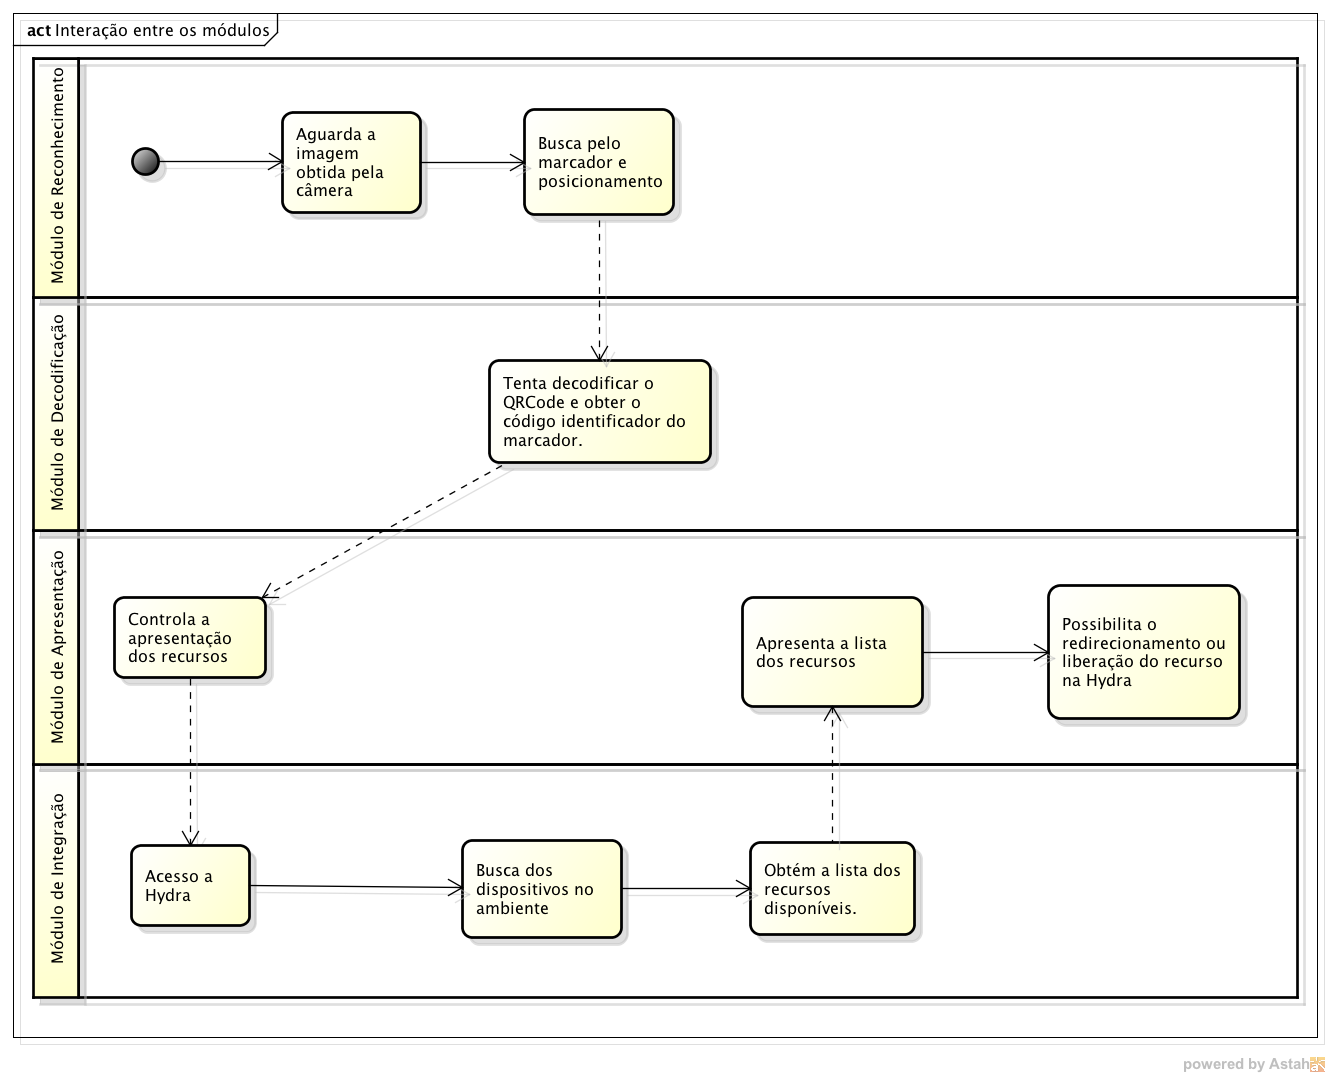
\includegraphics[scale=0.45]{figuras/cap4/interacao_modulos.png}
		\caption{\textit{Interação entre os módulos.}}
		\label{fig:interacao_modulos} 
	\end{figure}

	\section{Módulo de Reconhecimento}
\label{sec:modulo_reconhecimento}

	
	Neste módulo é realizada o reconhecimento dos marcadores bem como a obtenção de sua posição na
	imagem do ambiente. Este é notificado a cada imagem nova capturada pela câmera do dispositivo e de
	posse desta sua linha de execução inicia os passos apresentados na figura \ref{fig:processo_detect} e
	conforme descrito a seguir:
	
	\begin{figure}[h]
		\centering 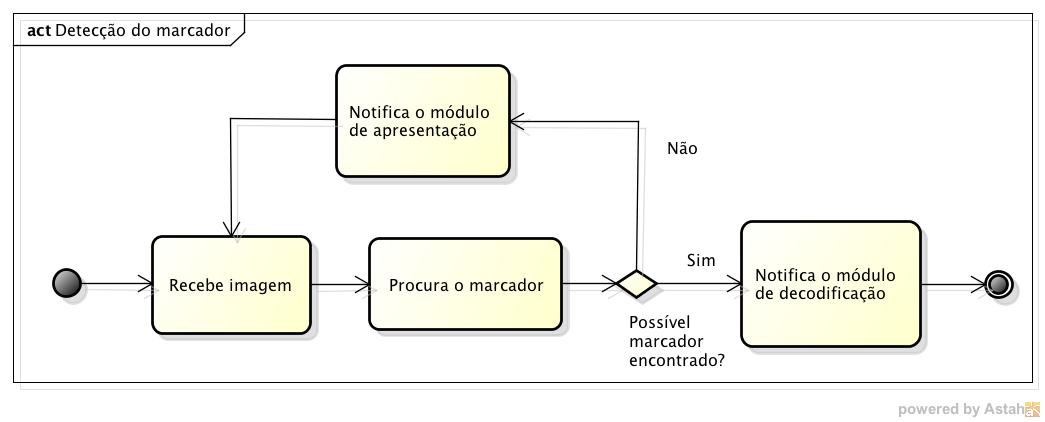
\includegraphics[scale=0.55]{figuras/cap4/processo_deteccao.png}
		\caption{\textit{Processos do Módulo de Reconhecimento.}}
		\label{fig:processo_detect} 
	\end{figure}
	
	\begin{enumerate}

	  \item A imagem obtida é convertida para escala de cinza com o intuito de se obter uma 
	  	homogeneidade da coloração dos \textit{pixels}. Desta forma a detecção de padrões ocorre de forma 
	  	facilitada.
	  
	  \item Utilizando a biblioteca OpenCV é realizada a correção de perspectiva da imagem, já que 
	  	o ângulo observado é distinto da figura esperada (vista frontal). Através da mesma biblioteca 
	  	é realizada a detecção de contornos, com base na borda negra do marcador, e determinação dos 
	  	quatro pontos que a delimitam.
	  	
	  \item Estima-se o posicionamento do marcador baseado nos quatro pontos não lineares
	  		identificados no passo anterior. Nesse procedimento também é obtido o ponto central da imagem,
	  		responsável pelo posicionamento correto do objeto virtual a ser sobreposto ao marcador.
	  
	  \item Para a obtenção da orientação do marcador foi utilizado o sensor de orientação disponível pelo
	  		\textit{smartphone}. A partir dessas informações é possível estimar o ângulo correto de visão
	  		do \textit{smartphone}, posicionando o objeto virtual corretamente.
	  		
	\end{enumerate} 
	
	Caso os quatro passos sejam executados com sucesso, tanto o marcador quanto sua posição seja obtida 
	com sucesso, estas informações são repassadas ao Módulo de Decodificação para que se prossiga com o fluxo 
	normal da aplicação. Caso contrário, é feita uma contagem para analisar se o marcador ainda está sendo 
	capturado pela câmera do celular. Se o processo em andamento atingiu a quantidade máxima de tentativas 
	consecutivas sem sucesso, o Módulo de Apresentação é notificado a respeito que nenhum marcador foi encontrado na 
	imagem, desta forma é possível atualizar a visão do usuário. Independente de ter ocorrido um reconhecimento, 
	o módulo voltará a aguardar	uma nova imagem para que um novo procedimento seja feito.
	
	Apesar da plataforma Android aceitar aplicações que sejam desenvolvidas utilizando a linguagem Java é
	possível combinar aplicações Java com aplicações e bibliotecas desenvolvidas em C/C++. Essa
	integração ocorre através do JNI (\textit{Java Native Interface}) suportada pelo 
	NDK \textit{(Native Development Kit)}. Tirando proveito deste suporte, este módulo integra-se com
	a solução elaborada para o reconhecimento através de uma conexão utilizando o JNI, devido ao fato
	do processo de reconhecimento utilizar a biblioteca \textit{OpenCV}, implementada utilizando a
	linguagem C.

	\section{Módulo de Decodificação}
\label{sec:modulo_decodificacao}

	Conhecendo a imagem do marcador encontrado cabe a este módulo extrair a informação representada por 
	ele. Para isto são utilizados marcadores QRCode ao qual representa o nome do dispositivo. Desta forma é 
	possível encontrar os recursos (\textit{drivers}) por este disponibilizados. Assim como o Módulo de Reconhecimento, 
	este módulo consiste em uma linha de execução própria e seu fluxo de execução ocorre conforme representado 
	na Figura \ref{fig:processo_decode} e descrito a seguir.
	
	\begin{figure}[htb]
		\centering 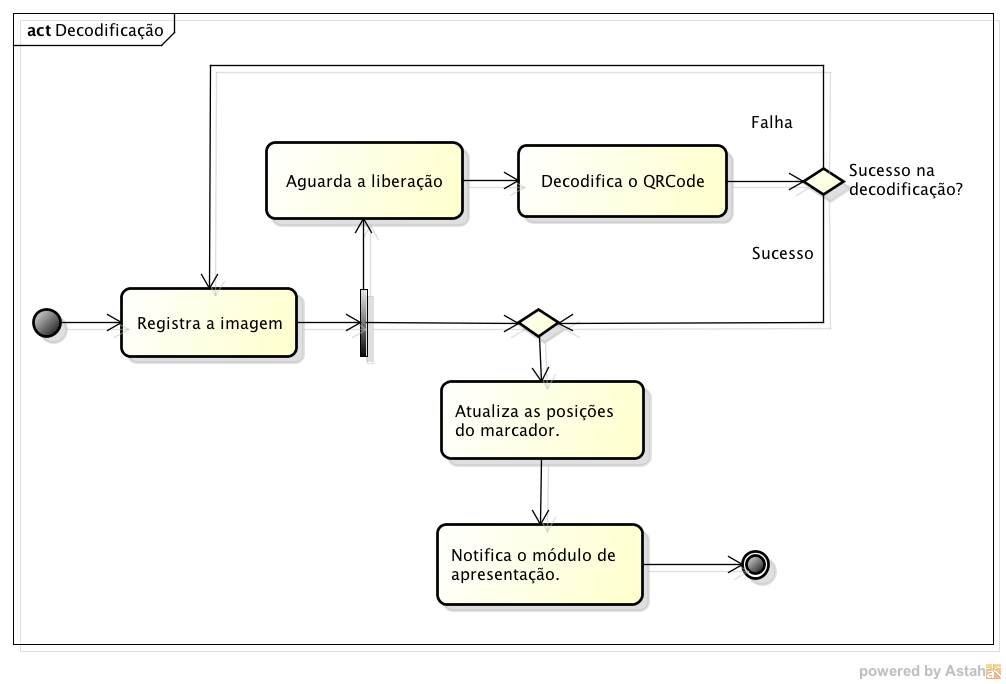
\includegraphics[scale=0.6]{figuras/cap4/processo_decodificacao.png}
		\caption{\textit{Processos do Módulo de Decodificação.}}
		\label{fig:processo_decode} 
	\end{figure}
	
	O Módulo de Decodificação é criado junto com o módulo de Reconhecimento, no entanto sua execução é 
	iniciada após o recebimento de algum marcador encontrado pelo Módulo de Reconhecimento. O marcador 
	recebido é registrado para que seja feito a atualização das informações a respeito da imagem recebida.
	Com o registro efetuado com sucesso é dado início ao processo de decodificação do marcador recebido. 
	Pelo fato do processo de reconhecimento ser mais rápido quando comparado ao processo de decodificação
	fez-se necessário a criação de um controle para que fosse garantido uma correta sincronização na 
	decodificação dos marcadores. Por essa razão, ocorrerá o descarte de qualquer marcador recebido enquanto 
	houver um processo de decodificação em execução. 
	
	Foi criado um Gerenciador com o propósito de centralizar todas as informações necessárias, de classes e 
	procedimentos, envolvidas no processo de decodificação. Ele age como uma interface entre o Módulo de 
	Decodificação e as aplicações responsáveis pela decodificação. A aplicação ZBar~\cite{zbar} foi utilizada 
	como ferramenta suporte ao processo de decodificação. Esta ferramenta é implementada utilizando a linguagem C. 
	Por essa razão a integração entre a aplicação ZBar com a ARHydra ocorre através do JNI. 
	
	As posições do marcador são atualizadas após o processo de decodificação ser finalizado com sucesso, ou seja, 
	houve êxito na obtenção do código de identificação do marcador analisado. Essa mesma etapa correspondente a  
	atualização das posições é feita quando um marcador é recebido do Módulo de Reconhecimento. Essa tarefa tem 
	um comportamento assíncrono devido o processo de decodificação ser um processo oneroso quando comparado dos 
	demais procedimentos separadamente. Por essa razão, enquanto houver um processo de decodificação em execução, as 
	posições referentes ao objeto virtual apresentado ao usuário são atualizadas com as informações recebidas
	pelos marcadores enviadas do Módulo de Reconhecimento. Após a atualização, essas informações são repassadas 
	ao Módulo de Apresentação para que as informações correspondentes ao marcador sejam atualizadas e apresentadas 
	ao usuário.
	
	Por outro lado, caso o processo de decodificação não consiga obter o código identificador correspondente ao 
	marcador analisado, o Módulo de Decodificação enviará uma notificação para o Módulo de Apresentando informando 
	a não possibilidade de detecção do código identificador do marcador, desta forma é possível atualizar a visão
	do usuário. Após a conclusão dessa notificação, o Módulo de Decodificará aguardará o recebimento da próxima 
	imagem enviada pelo Módulo de Reconhecimento, reinicializando todos os procedimentos até aqui apresentados 
	para este módulo.
	
	
	\section{Módulo de Integração} 
\label{sec:modulo_integracao}

	Na composição do objeto virtual é necessário reunir informações relevantes sobre a disponibilidade dos 
	recursos provido pelo dispositivo escolhido. O Módulo de Integração é responsável pela integração da 
	ARHydra com a Hydra com o propósito de criar um canal de comunicação entre essas duas aplicações. Esta 
	integração é feita através de \textit{drivers} de comunicação, conforme	estabelecido pela DSOA. 
	
	Quando um recurso apresentado pelo dispositivo é selecionado faz-se necessário informar a Hydra	qual 
	recurso fora escolhido. Esse canal externo de comunicação entre as aplicações não é fornecida pelo 
	\textit{uOS} de forma nativa. Por essa razão, a arquitetura inicial da Hydra 
	não implementou nenhuma forma para o recebimento de requisições externas. Permite apenas a interação 
	via terminal de aplicação, ou seja, sem acesso por outras aplicações. Desta forma, para o usuário 
	redirecionar algum recurso, ele terá que ir até o dispositivo executando a Hydra e prover o 
	redirecionamento de forma manual. Para realizar essa comunicação foi desenvolvido um~\textit{driver} 
	na Hydra que possibilitasse o recebimento de requisições externas. O envio das requisições, bem como
	o recebimento das respostas realizadas pelas mesmas, decorrentes dessa comunicação, ocorre através do 
	Módulo de Integração.  

	Para economizar recursos do \textit{smartphone}, a obtenção da informação de quais dispositivos
	estão disponíveis dentro do ambiente inteligente fica sob responsabilidade da Hydra, ao qual implementará
	mecanismos para identificação dos dispositivos no ambiente através da utilização de radares. A ARHydra 
	possui um mecanismo de agendamento para que essa informação seja atualizada. Com a periodicidade de 60 segundos, 
	o Módulo de Integração envia informações para a Hydra requisitando quais são os dispositivos que estão 
	ativos dentro do ambiente.
	
	\section{Módulo de Apresentação}
\label{sec:modulo_apresentacao}

	Após o marcador ser reconhecido e identificado, o Módulo de Apresentação fica responsável por
	apresentar ao usuário todos os recursos disponíveis do dispositivo selecionado. São aceitos os
	mesmos recursos compatíveis com a Hydra: câmera, \textit{mouse}, teclado ou tela. Os recursos são
	visualizados através de um objeto virtual, ao qual é apresentado na tela. Este é representado
	através de um retângulo onde é exibido o nome do dispositivo e os recursos por ele
	disponibilizados. Na figura \ref{fig:objeto_virtual}, podemos observar um caso onde temos o 
	dispositivo iMacDevice que disponibiliza os seus recursos de câmera,~\textit{mouse}, tela e teclado.

	
	\begin{figure}[htb]
		\centering 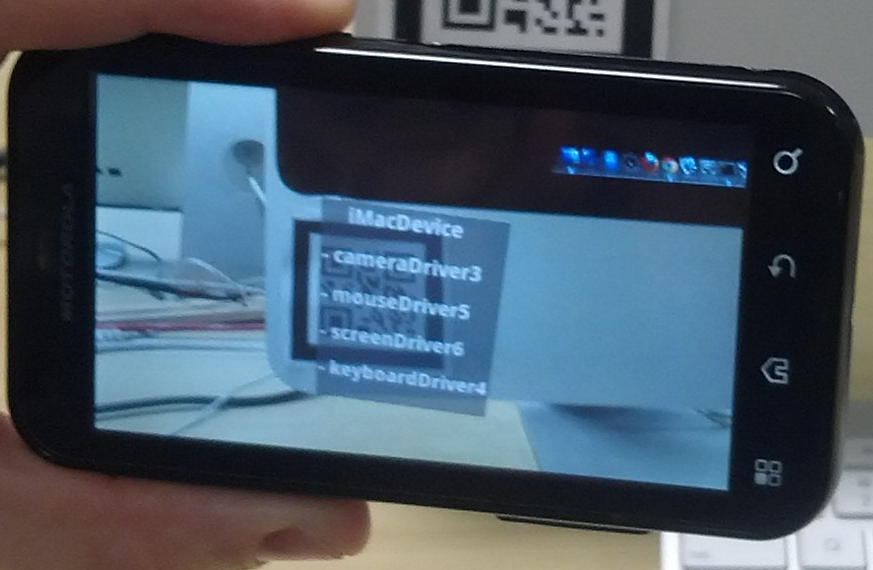
\includegraphics[scale=0.3]{figuras/cap4/objeto_virtual.png}
		\caption{\textit{Objeto virtual.}}
		\label{fig:objeto_virtual} 
	\end{figure}
	
	Para interagir com o dispositivo basta ao usuário tocar a tela sobre o objeto que o representa.
	Desta forma é exibida uma nova tela onde é possível controlar o uso dos recursos do dispositivo.
	Possibilitando ao usuário selecionar o redirecionamento ou liberação conforme desejado. A 
	figura~\ref{fig:listagem_recursos} mostra o detalhamento dos recursos disponíveis ao usuário no 
	dispositivo. Os recursos de teclado e \textit{mouse} já estão sendo redirecionados para a Hydra, 
	enquanto os demais estão disponíveis para serem utilizados pela mesma.
	
	
	\begin{figure}[htb]
		\centering 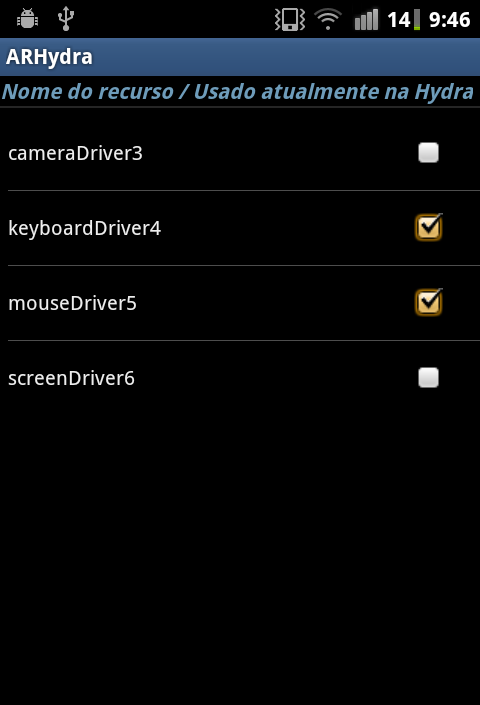
\includegraphics[scale=0.35]{figuras/cap4/listagem_recursos.png}
		\caption{\textit{Listagem dos recursos.}}
		\label{fig:listagem_recursos} 
	\end{figure}
	
	O \textit{framework} DroidAR \cite{droidar} foi utilizado para facilitar a renderização dos objetos 
	na tela. Para o gerenciamento desses objetos virtuais fez-se necessário a criação de uma classe 
	responsável pela criação, reposicionamento e deleção desses objetos. Essa classe recebe informações
	dos Módulos de Reconhecimento e Decodificação para determinar a ação a ser executada. A interação
	desse controle com os demais módulos é apresentado na figura~\ref{fig:condicoes_objeto}.

	\begin{figure}[htb]
		\centering 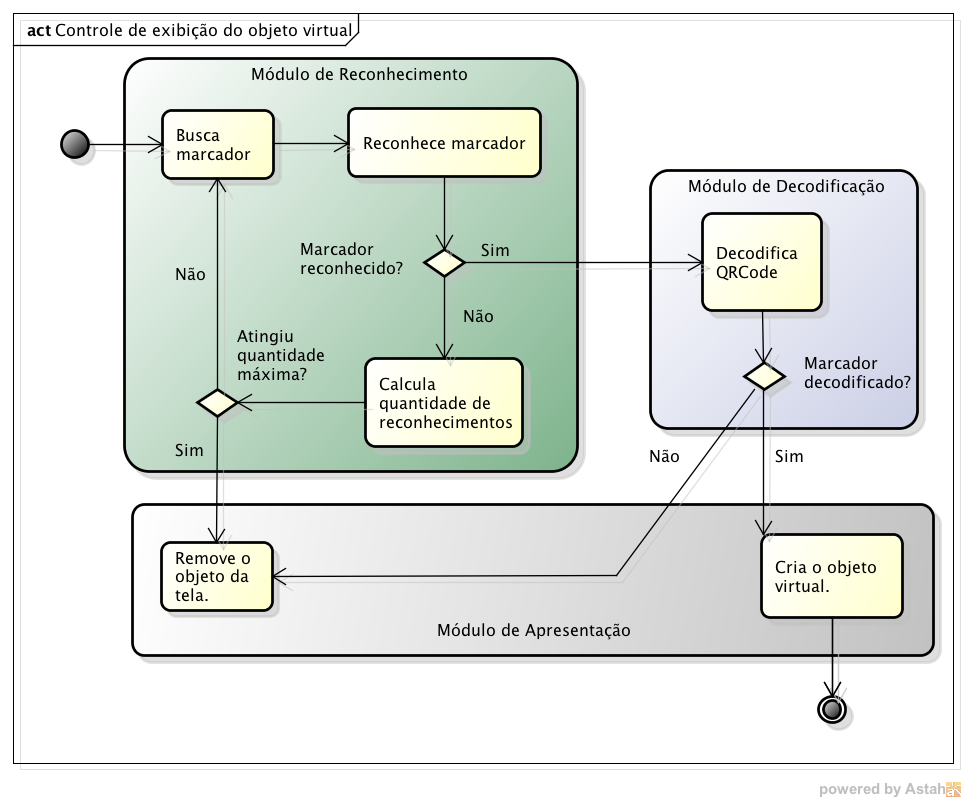
\includegraphics[scale=0.55]{figuras/cap4/condicoes_objeto.png}
		\caption{\textit{Condições para visualização do objeto virtual.}}
		\label{fig:condicoes_objeto} 
	\end{figure}

	Desta maneira, o controle de exibição dos objetos virtuais possibilita uma correta visualização
	dos recursos disponíveis pelos dispositivos. De modo que somente os recursos de um dispositivo
	sejam apresentados por vez.
	

	\section{Hydra \textit{Driver}}
\label{sec:hydradriver}

	A aplicação Hydra foi concebida para ter seu controle realizado pelo usuário diretamente na máquina de 
	onde os recursos seriam direcionados. Desta forma, não seria possível que outros dispositivos solicitassem 
	que um novo redirecionamento seja realizado. Para superar esta limitação foi desenvolvido um~\textit{driver} 
	denominado~\textit{HydraDriver} que disponibiliza as opções de interação da Hydra no~\textit{Smart Space}.
	
	Este recurso visa replicar as mesmas capacidades disponíveis na interface gráfica da aplicação original 
	sendo composto por um conjunto de três serviços síncronos:
	
	\begin{enumerate}
	  \item \textbf{Redirecionamento do recurso:} Com este serviço é possível redirecionar um recurso da 
	  	máquina para um disponível em outro dispositivo.
	  
	  \item \textbf{Liberação do recurso:} Informado o recurso desejado e o dispositivo a ele relacionado, 
	  	é finalizado o redirecionamento existente entre eles.
	  
	  \item \textbf{Uso do recurso:} Retorna as informações acerca do recurso local. Nestas informações 
	  	é possível observar se ele está em uso no momento e para qual dispositivo está sendo redirecionado.
	  
	\end{enumerate}	
	

	\section{Testes}
	
	A operação da aplicação ARHydra está diretamente relacionada ao tempo que esta necessita para levar a informação ao 
	seu usuário. Com o objetivo de medir este tempo foram realizados testes onde se variou a distância do marcador 
	bem como o equipamento utilizado. Os dados foram analisados com relação a execução completa dos três componentes 
	envolvidos na operação (reconhecimento, decodificação e apresentação). Estes testes foram realizados no ambiente do 
	LAICO (LAboratorio de Sistemas Integrados e COncorrentes), situado no Departamento de Ciências da Computação da 
	Universidade de Brasília. Foram utilizados dois~\textit{smartphones} distintos, um Motorola Defy e um 
	Sansung Galaxy SIII, de forma a avaliar a influência da qualidade da câmera e do processamento durante o uso. O Motorola 
	Defy possui as seguintes especificações: processador Cortex-A8 de 800 MHz, 512 MB de memória RAM, resolução de tela 
	de 480 x 854~\textit{pixels}, GPU (\textit{Graphics Processing Unit}) PowerVR SGX530 e câmera com resolução de 5MP. 
	O Sistema Operacional testado nesse dispositivo foi o Android 2.3.7 com~\textit{firmware} CyanogenMod 7.2. Já o 
	\textit{smartphone} Samsung Galaxy SIII possui processador Quad-core 1.4 GHz Cortex-A9, 1GB de memória RAM, 
	resolução da tela de 720 x 1280~\textit{pixels}, GPU Mali-400MP, câmera com resolução de 8MP e sistema operacional 
	Android 4.0.4.

\subsection{Reconhecimento dos marcadores}
	
	Foram executados conjuntos de testes com o objetivo de mensurar o tempo gasto no processo de
	reconhecimento do marcador proposto. O tempo de reconhecimento é composto pela soma dos tempos gasto
	na identificação das bordas do marcador, do processo de decodificação do QRCode, da obtenção dos
	dados (via integração com a Hydra) referentes ao marcador selecionado e da apresentação dos
	recursos ao usuário. Deste modo, foram propostos testes que realizassem as seguintes medições:
		
	\begin{enumerate}
	  \item \textbf{Medição do tempo do primeiro reconhecimento:} Tempo com que o
	  		marcador é reconhecido pela primeira vez após a aplicação ARHydra ser inicializada;
	  
	  \item \textbf{Medição do tempo de recorrência:} Tempo com que a aplicação gasta para
	  		reconhecer um marcador de forma recorrente, conforme a câmera é movimentada sem que a mesma
	  		perca a visualização do marcador;
	  
	  \item \textbf{Medição do tempo de reconhecimento após o marcador não estar mais no campo de visão da
	  		câmera do \textit{smartphone}:} Tempo médio necessário para que a aplicação
	  		reconheça um novo marcador após o usuário perder o campo de visão do marcador
	  		no~\textit{smartphone}.
	  		
	  \item \textbf{Taxa de erros:} Este valor representa o percentual das ocorrências com que a
			aplicação ARHydra deixou de identificar o marcador quando este estava sendo capturado pela câmera
			do~\textit{smartphone}.
	   
	   \item \textbf{Taxa de não decodificação:} Este valor representa a porcentagem média de falha nas decodificações 
	   		do QRCode inseridos no marcador. As ocorrências nesta taxa são contabilizadas quando um marcador é reconhecido
	   		porém não é feita a decodificação do QRCode pelo Módulo de Decodificação. Esse valor varia de acordo 
	   		com a aplicação responsável pela decodificação, o nível de tolerância a falhas utilizada no QRCode, a 
	   		qualidade da obtenção das imagens pelo dispositivo e a distância entre o marcador e o~\textit{smartphone}. 
	
	\end{enumerate}
	
	A aplicação ARHydra oferece suporte, presente no Módulo de Decodificação, para a utilização de diversos 
	aplicativos ao qual disponibilizem o recurso de decodificação de QRCode's. Através desse suporte foram 
	realizados testes que permitiram estabelecer um comparativo de desempenho entre essas diversas aplicações 
	utilizadas. A fim de obter esse comparativo, as aplicações ZBar~\cite{zbar} e ZXing~\cite{zxing} foram	
	utilizadas nos referidos testes.
	
	Uma outra informação importante a ser definida refere-se ao estabelecimento de uma distância máxima
	para o reconhecimento destes marcadores. Este valor pode variar de acordo com a aplicação
	utilizada no processo de decodificação, considerando as limitações envolvidas no recolhimento das
	informações necessárias para a decodificação mesmo quando os QRCode's apresentarem níveis de
	tolerância a falhas. Desta maneira, para o estabelecimento desse valor, os testes propostos foram
	executados para diferentes distâncias.
	
	As taxas de erros e de não decodificação estão diretamente relacionadas a qualidade da imagem obtida. No entanto,
	esta qualidade não diz respeito somente a resolução da câmera utilizada, outros fatores podem influenciar no
	reconhecimento do marcador. Dentre estes pode-se citar a qualidade das lentes e o algoritmo utilizado na compressão 
	das imagens, possibilitando que seja obtido resultados diferentes para cenários semelhantes, quando estes 
	resultados são coletados utilizando dispositivos dotados de diferentes câmeras. Um outro ponto importante 
	para se garantir esta qualidade está no controle de luminosidade implementado pelas câmeras. Para minimizar esses 
	problemas apresentados é possível ser implementado etapas de pré-processamento da imagem para melhorar a qualidade
	dessa imagem obtida.
	
\subsubsection{Especificações do Marcador}

	O marcador foi construído baseando nas especificações apresentadas pelo QRCode
	(seção~\ref{sec:simbolos_bidimensionais}) e nas dimensões necessárias voltadas para o módulo de
	reconhecimento validar o marcador. Também deve ser considerado a inserção desses marcadores no ambiente de forma menos
	intrusiva possível, mas que suas caraterísticas possibilitem seu reconhecimento.
	
	A Figura~\ref{fig:dimensoes_marcador} apresenta as dimensões adotadas na construção desses
	marcadores. O QRCode é envolvido por uma moldura, com bordas no valor experimental de 0,8 centímetros, 
	para que o módulo de reconhecimento consiga validar e estabelecer as informações de
	posicionamento referentes ao marcador e o módulo de decodificação realize com sucesso a decodificação
	do QRCode.
	
	\begin{figure}[htb]
		\centering 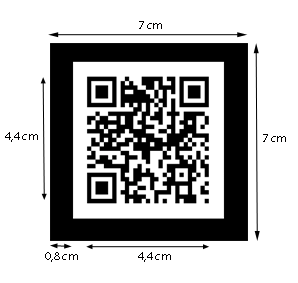
\includegraphics[scale=0.8]{figuras/cap4/dimensoes_marcador.png}
		\caption{\textit{Dimensões do marcador.}}
		\label{fig:dimensoes_marcador} 
	\end{figure}
	
\subsection{Resultados}
\label{sec:resultados}

	Os conjuntos de testes foram executados a uma distância inicial de 50
	centímetros, referente a distância entre o marcador e a aplicação ARHydra executada
	no~\textit{smartphone}, sendo esta aumentada gradativamente em 10 centímetros até atingir o valor 
	de 1 metro. Foram executados os seguintes testes:
	
	\begin{itemize}
	  \item Desempenho e qualidade da obtenção da imagem: Neste teste foi utilizado dois
	  		~\textit{smartphones} com o propósito de estabelecer a diferença de desempenho da aplicação
	  		ARHydra, bem como apresentar o comparativo entre taxas de reconhecimento e não decodificação 
	  		do QRCode para cada~\textit{smartphone} utilizado.
	  
	  \item Suporte a diversas aplicações de decodificação do QRCode: Neste teste foi validado o suporte 
	  		oferecido pela ARHydra para a utilização de diversos aplicativos cujo propósito seja a 
	  		decodificação de QRCodes.
	  		
	  \item Influência da tolerância a falhas do QRCode: Este permite medir a influência dos níveis de 
	  		tolerância a falhas aplicados ao QRCode e sua relação com a taxa de não decodificação.
	  			  
	\end{itemize}

\subsubsection{Teste de desempenho e qualidade na obtenção da imagem}
\label{sec:testesDesempenho}

 
	Um dos objetivos para este teste é comparar o desempenho da aplicação ARHydra utilizada nos dispositivos mencionados 
	anteriormente, com o propósito de  mensurar a diferença nos tempos de reconhecimento do marcador, sendo esta 
	influenciada diretamente pela capacidade de processamento, processador e~\textit{GPU}, de cada dispositivo. O outro 
	objetivo consiste em analisar a influência da qualidade da imagem obtida pela câmera, destes dispositivos, estabelecendo 
	um comparativo entre as taxas de erro e não decodificação.
	
	Para a execução do teste foram realizadas vinte medições para a primeira aparição, duzentas medições para as recorrências 
	e cinquenta medições para o reconhecimento ao perder o marcador. Os resultados dessas medições são apresentados nos 
	gráficos das Figuras~\ref{fig:testeCompDesempenho} e \ref{fig:testeCompTaxas}.
	
	\begin{figure}[htb] 
		\centering 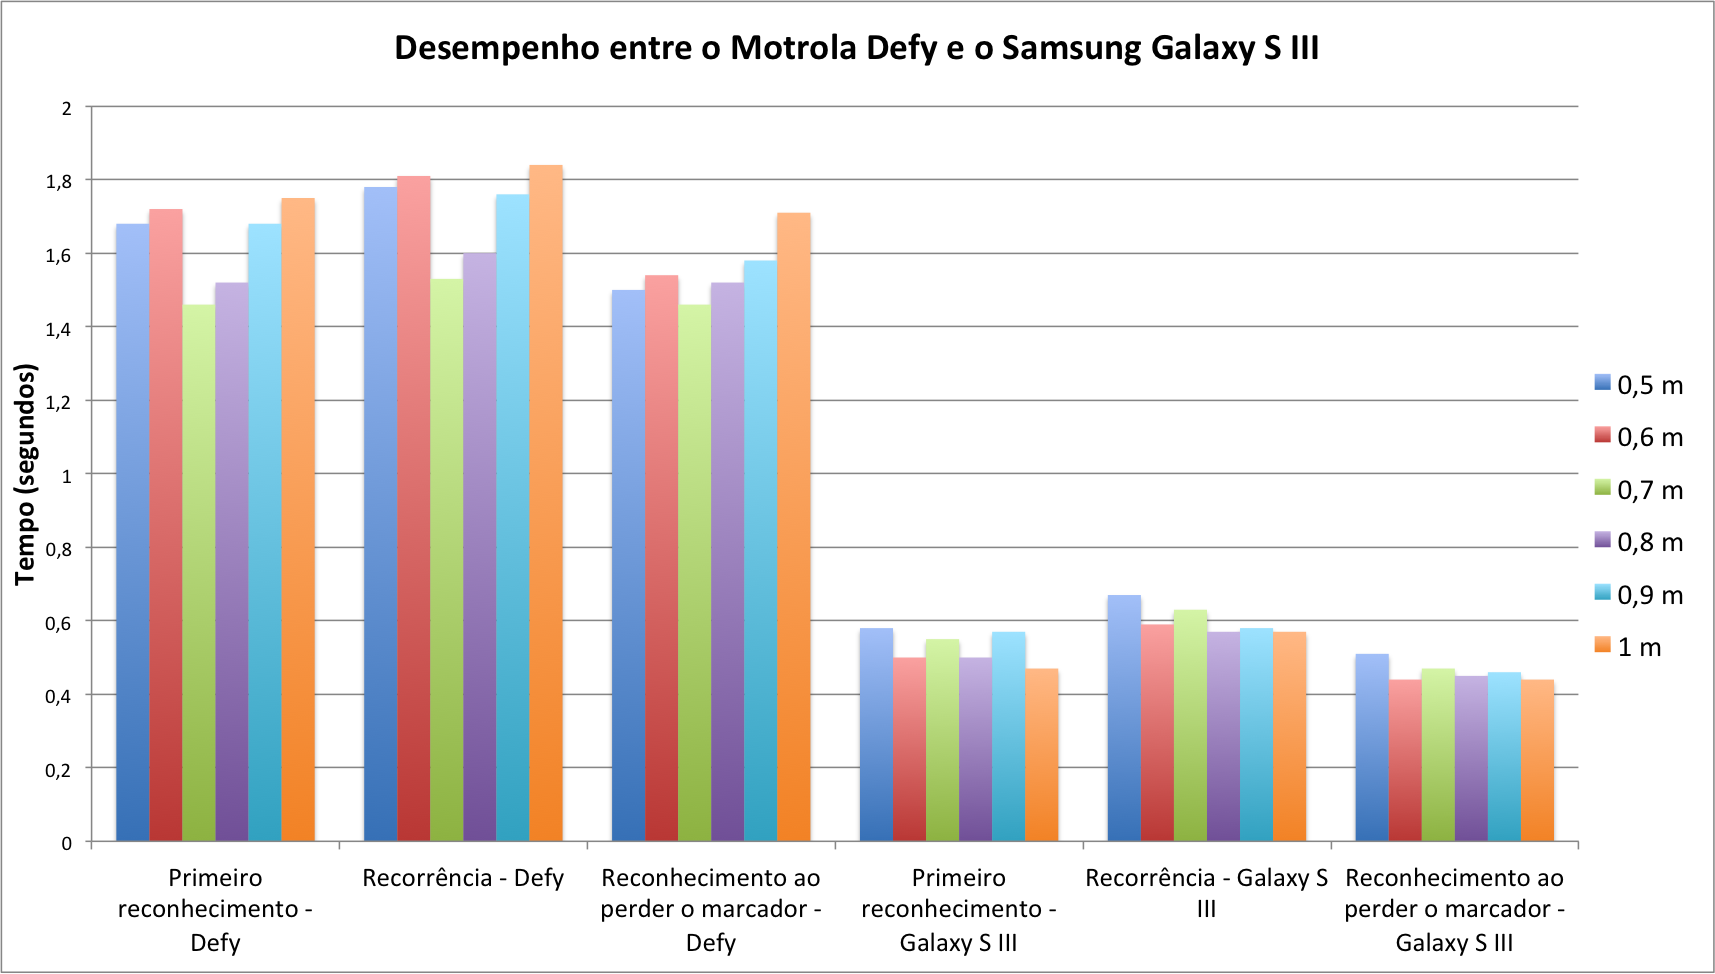
\includegraphics[scale=0.55]{figuras/cap4/grafico_desempenho.png}
		\caption{\textit{Comparativo de desempenho da aplicação ARHydra entre os dispositivos Motorola Defy e 
							Samsung Galaxy SIII.}}
		\label{fig:testeCompDesempenho} 
	\end{figure}
	
	
	A Figura \ref{fig:testeCompDesempenho} apresenta o resultado que mede o desempenho dos dispositivos. Ela mostra que o 
	dispositivo Galaxy SIII obteve melhor desempenho, sendo mais rápido no reconhecimento dos marcadores, devido a diferença 
	na capacidade de processamento, processador e~\textit{GPU}, presente no processador do Galaxy SIII. Desta forma, 
	quanto maior for a capacidade de processamento do dispositivo menor será o tempo gasto pela aplicação ARHydra reconhecer
	os marcadores.   
	
	Os tempos obtidos no primeiro reconhecimento foram inferiores quando comparados ao tempo gasto na recorrência, em ambos 
	os dispositivos, por causa da baixa quantidade de imagens a serem processadas ou descartadas pelos módulos de 
	reconhecimento,	decodificação e apresentação após a captura das imagens ser inicializada. Adicionalmente, a 
	aplicação ARHydra não apresenta um mecanismo de histórico de reconhecimentos ocasionando com que cada 
	reconhecimento concluído com sucesso seja considerado um novo reconhecimento, onerando assim o tempo de recorrência. 
	
	\begin{figure}[htb] 
		\centering 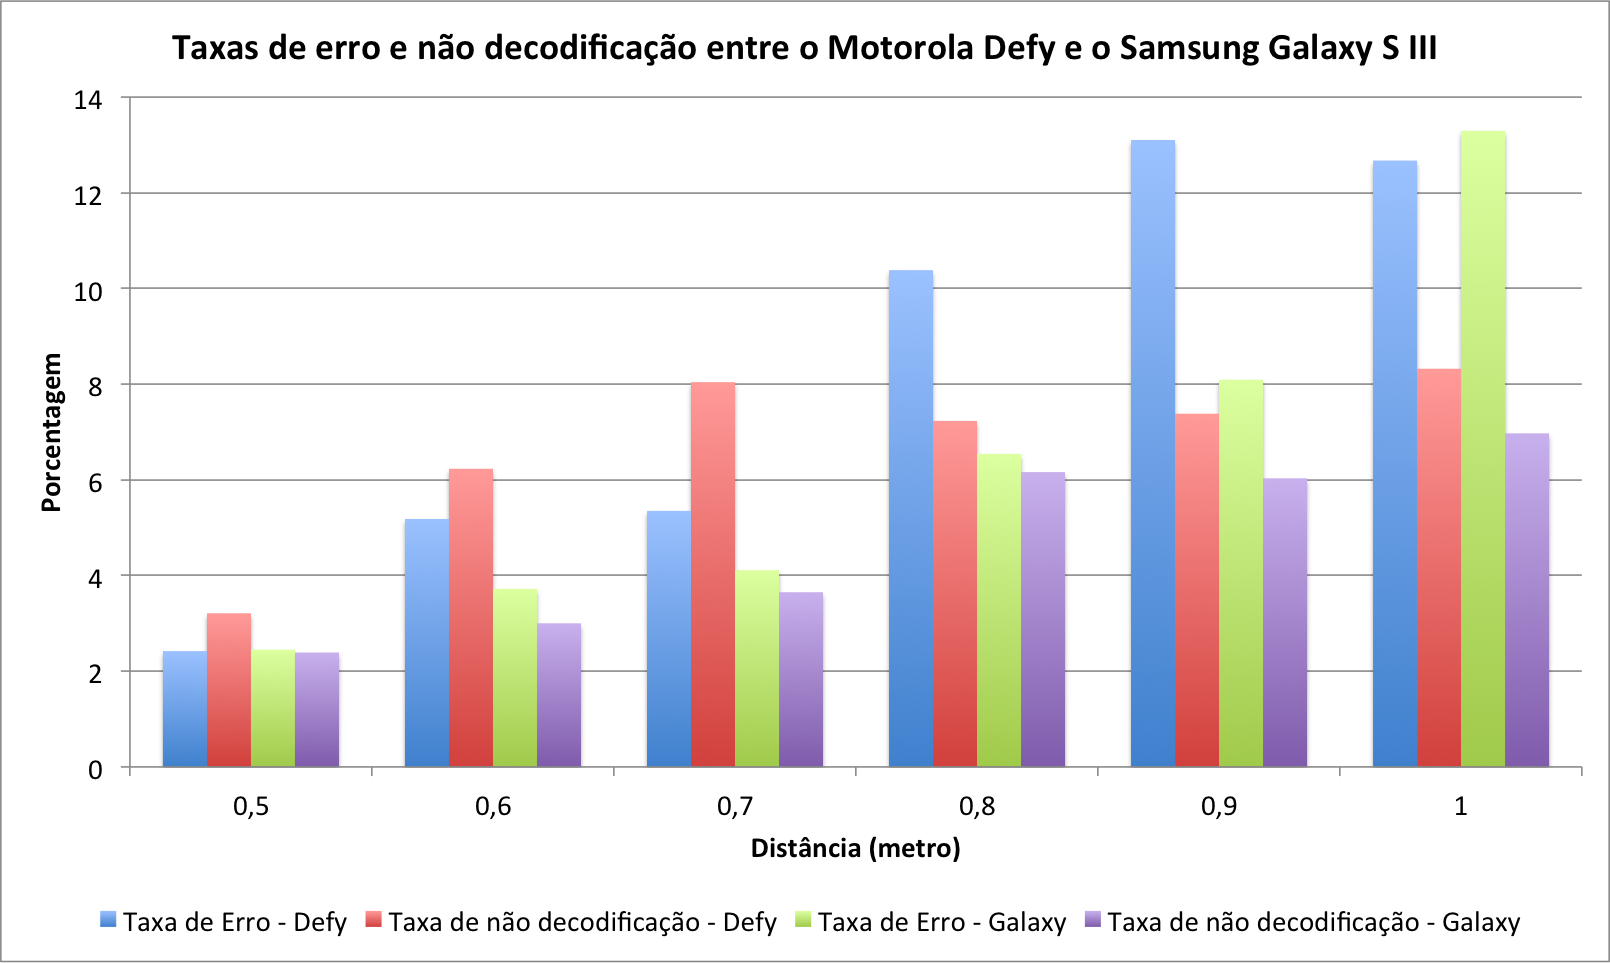
\includegraphics[scale=0.55]{figuras/cap4/grafico_taxas_defy_s3.png}
		\caption{\textit{Comparativo entre as taxas de erro e de não decodificação da aplicação ARHydra entre os 
						dispositivos Motorola Defy e Samsung Galaxy SIII.}}
		\label{fig:testeCompTaxas} 
	\end{figure}
	
	A Figura~\ref{fig:testeCompTaxas} apresenta as Taxa de Erros e Taxa de não decodificação. Novamente o Galaxy SIII 
	mostrou superioridade na maioria das distâncias avaliadas. Esses resultados demonstram a influência da qualidade 
	da imagem capturada em relação as taxas aqui apresentadas. Não levando em consideração as etapas voltadas ao 
	pré-processamento de imagens que possam ser implementadas na ARHydra, conclui-se então que quanto maior for a qualidade da 
	câmera (resolução, qualidade das lentes, algoritmo utilizado na compressão das imagens, controle de luminosidade, etc), 
	juntamente com a melhoria na qualidade dos valores recebidos pelo sensor de orientação do~\textit{smartphone}, menores 
	serão as taxas de erro e decodificação apresentadas na ARHydra. 
	
\subsubsection{Suporte a diversas aplicações de decodificação do QRCode}

	A ARHydra permite a integração de diferentes mecanismos para a decodificação de QRCodes a serem utilizados no Módulo 
	de decodificação. Na atual versão da aplicação é permitido utilizar tanto a implementação fornecida pelo ZBar e o 
	ZXing para esta tarefa. Tomando esta flexibilidade como base, foram realizados testes para verificar o comportamento 
	fornecido por cada um destes. 
	
	Para estes testes foi utilizado o~\textit{smartphone} de melhor capacidade, o Samsung Galaxy SIII, de forma que o 
	nível de tolerância a falhas do QRCode foi ajustado para o modo~\textit{Quality}. Neste teste 
	foram obtidas quinhentas medições por posição em cada implementação. Os resultados obtidos podem ser observados na 
	Figura~\ref{fig:testeSuporte}.
	
	\begin{figure}[htb] 
		\centering 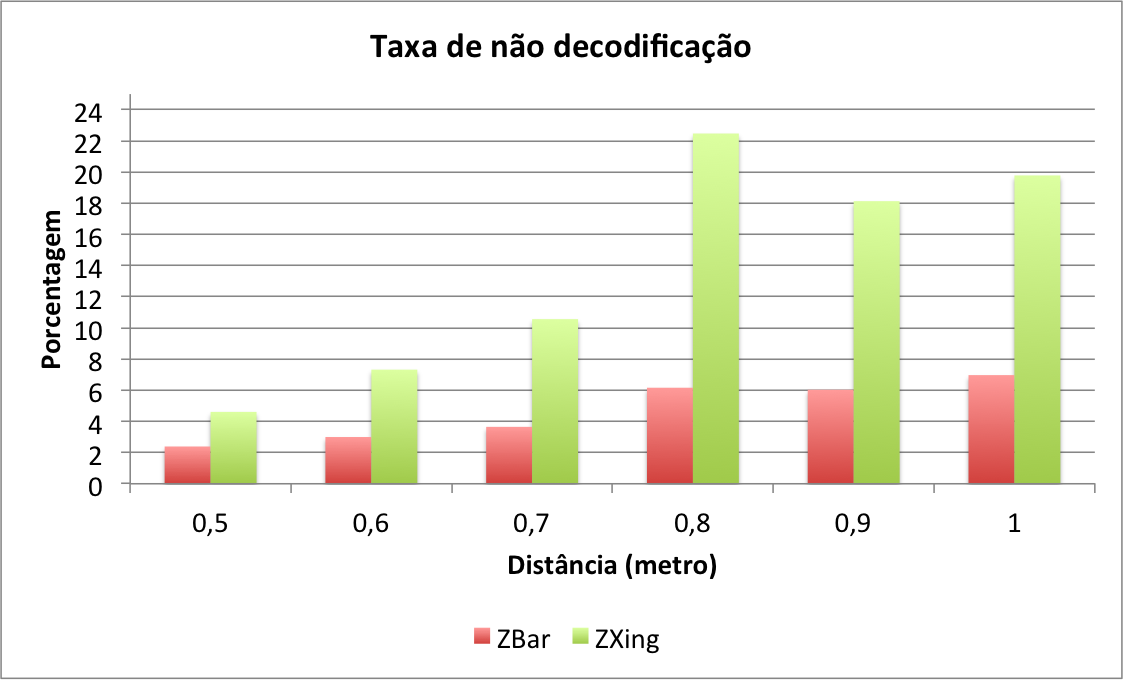
\includegraphics[scale=0.75]{figuras/cap4/grafico_suporte.png}
		\caption{\textit{Taxa de não decodificação para as aplicações ZBar e ZXing.}}
		\label{fig:testeSuporte} 
	\end{figure}
	
	Os resultados apresentados indicam que a implementação ZBar apresenta taxas de não decodificação mais baixas do 
	que a ZXing. Na maioria das distâncias analisadas, ambas as aplicações apresentaram aumento em suas taxas a 
	medida com que a distância fosse aumentada. A diferença apresentada nos resultados está relacionado ao algoritmo 
	utilizado por essas aplicações, porém não foi possível obter informações a respeito da implementação dos mesmos.
	
	
\subsubsection{Influência da tolerância a falhas do QRCode}

	%Estes níveis tem por objetivo facilitar a decodificação do QRCode, porém o formato do 
	%local de armazenamento de seu conteúdo varia de acordo com seu nível de tolerância a falhas implementado.
	
	Como visto na seção \ref{sec:simbolos_bidimensionais}, os QRCodes podem ser compostos por quatro níveis de 
	tolerância a falhas. Este conjunto de testes por sua vez, visa estabelecer um parâmetro de qual nível seria 
	melhor aplicado à aplicação ARHydra, uma vez que a longa distâncias a câmera não consegue capturar os pontos 
	do QRCode, impossibilitando	assim sua decodificação. 
	
	Para análise dos resultados foram realizadas quinhentas medições para cada distância, sendo esta 
	repetida para todos os níveis de tolerância a falhas. Por fim, o módulo de decodificação foi configurado 
	para utilizar a	aplicação ZBar nos testes mencionados, devido suas melhores taxas obtidas no teste anterior. 
	
	\begin{figure}[htb]
		\centering 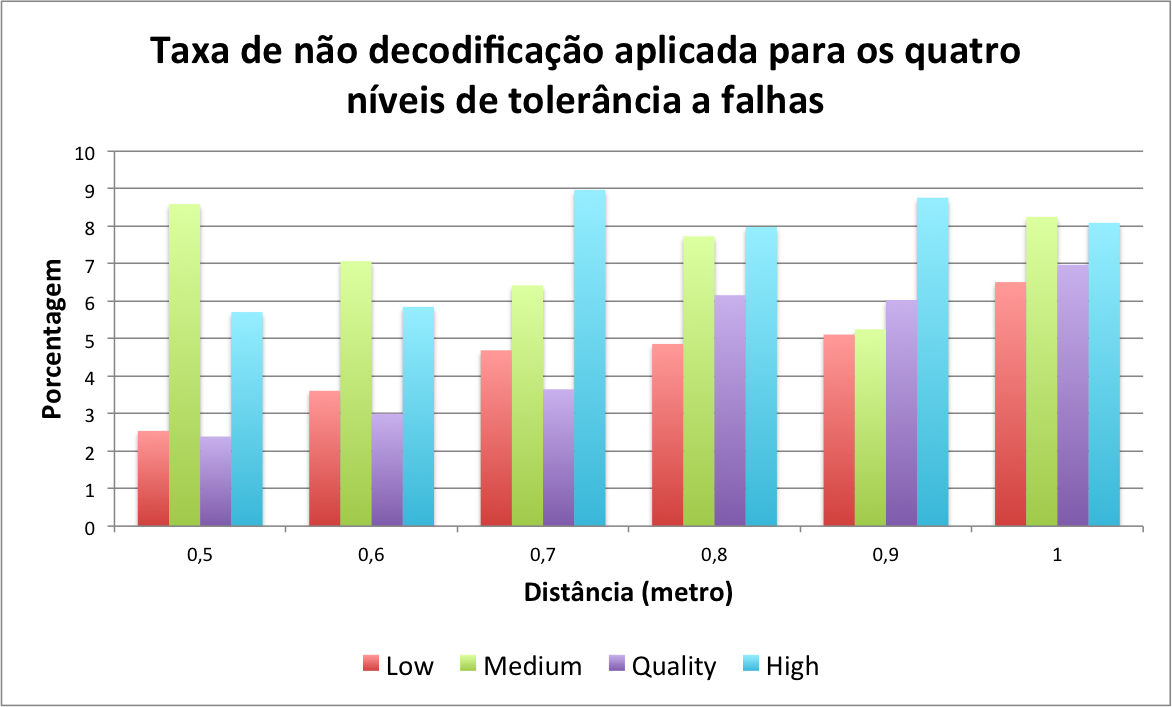
\includegraphics[scale=0.75]{figuras/cap4/grafico_nivel_decode.png}
		\caption{\textit{Nível da taxa de não decodificação aplicado sobre a influ{\^e}ncia da toler{\^a}ncia a falhas do QRCode.}}
		\label{fig:testeNivelDecode} 
	\end{figure}
	
	A Figura \ref{fig:testeNivelDecode} apresenta os resultados para este teste. Estes níveis possuem percentuais de 
	recuperação a falhas conforme a Tabela~\ref{tab:nivelFalha}. Os marcadores, quando ajustados aos 
	níveis~\textit{Low} e~\textit{Quality}, obtiveram melhores resultados comparado aos demais níveis. Embora, as taxas 
	de todos os níveis tenham apresentado aumento à medida que o dispositivo se afastava do marcador em questão. Quando 
	os níveis~\textit{Low} e~\textit{Medium} são comparados, é possível observar que o formato de seus campos responsáveis
	pela estruturação do QRCode, mesmo quando a diferença na porcentagem da tolerância a falhas é pequena, interfere na 
	obtenção dos pontos	internos ao código, ocasionando uma variação muito grande na taxa de não decodificação. 
	Esse mesmo comportamento é observado para os níveis~\textit{Quality} e~\textit{High}. 
	
	A medida com que é elevado o nível de tolerância a falhas há um aumento da quantidade de informação a ser armazenada
	para cobrir a porcentagem de informação que pode ser recuperada. No entanto, o espaço ocupado pelo QRCode, no marcador 
	utilizado, permaneceu o mesmo, independente do nível de recuperação a falhas aplicado. Desta forma, quanto maior o nível de 
	recuperação a falhas utilizado mais complexo será a decodificação do marcador utilizado. A partir dos resultados 
	analisados, conclui-se que o nível~\textit{Low} de tolerância a falhas é o que melhor se aplica para utilização na 
	aplicação ARHydra para as distâncias analisadas. 
	
	
	
		 
	

